% \documentclass[aspectratio=169,notes]{beamer}
\documentclass[aspectratio=169]{beamer}
\usetheme[faculty=phil]{fibeamer}
\usepackage{polyglossia}
\setmainlanguage{english} %% main locale instead of `english`, you
%% can typeset the presentation in either Czech or Slovak,
%% respectively.
\setotherlanguages{russian} %% The additional keys allow
%%
%%   \begin{otherlanguage}{czech}   ... \end{otherlanguage}
%%   \begin{otherlanguage}{slovak}  ... \end{otherlanguage}
%%
%% These macros specify information about the presentation
\title[Introduction to Robotics (In2Ro)]{Introduction to Robotics, Lecture 2} %% that will be typeset on the
\subtitle{Direct kinematics and DH notation 
\\ Analytical inverse kinematics \\ Numerical methods and workspaces  } %% title page.
\author{Oleg Bulichev}
%% These additional packages are used within the document:
\usepackage{ragged2e}  % `\justifying` text
\usepackage{booktabs}  % Tables
\usepackage{tabularx}
\usepackage{tikz}      % Diagrams
\usetikzlibrary{calc, shapes, backgrounds, trees, positioning, arrows.meta}
\usetikzlibrary{decorations.pathreplacing,calligraphy,calc,graphs}
\usepackage{amsmath, amssymb}
\usepackage{url}       % `\url`s
\usepackage{listings}  % Code listings
\usepackage{floatrow}
\usepackage{subcaption}
\usepackage{mathtools}
\usepackage{todonotes}
\usepackage{fontspec}
\usepackage{multicol}
\usepackage{pdfpages}
\usepackage{wrapfig}
\usepackage{qrcode}
\usepackage{animate}
\usepackage{booktabs}
\usepackage{multirow}
\usepackage{graphicx}
\usepackage{colortbl}

\graphicspath{{resources/}}
\frenchspacing

\setbeamertemplate{caption}{\raggedright\insertcaption\par}
\usetikzlibrary{graphs}

% \usepackage[backend=biber,style=ieee,autocite=footnote]{biblatex}
% \addbibresource{biblio.bib}
% \DefineBibliographyStrings{english}{%
%   bibliography = {References},}

\newcommand{\oleg}[2][] {\todo[color=red, #1] {OLEG:\\ #2}}
\newcommand{\fbckg}[1]{\usebackgroundtemplate{\includegraphics[width=\paperwidth]{#1}}}%frame background

\usepackage[framemethod=TikZ]{mdframed}
\newcommand{\dbox}[1]{
\begin{mdframed}[roundcorner=3pt, backgroundcolor=yellow, linewidth=0]
\vspace{1mm}
{#1}
\vspace{1mm}
\end{mdframed}
}

\begin{document}
\setlength{\abovedisplayskip}{0pt}
\setlength{\belowdisplayskip}{0pt}
\setlength{\abovedisplayshortskip}{0pt}
\setlength{\belowdisplayshortskip}{0pt}

\fbckg{fibeamer/figs/title_page.png}
\frame[c]{\setcounter{framenumber}{0}
    \usebeamerfont{title}%
    \usebeamercolor[fg]{title}%
    \begin{minipage}[b][6.5\baselineskip][b]{\textwidth}%
        \textcolor{black}{\raggedright\inserttitle}
    \end{minipage}
    % \vskip-1.5\baselineskip

    \usebeamerfont{subtitle}%
    \usebeamercolor[fg]{framesubtitle}%
    \begin{minipage}[b][3\baselineskip][b]{\textwidth}
        \raggedright%
        \insertsubtitle%
    \end{minipage}
    \vskip.25\baselineskip
}

\fbckg{fibeamer/figs/common.png}

\begin{frame}[t]{What Kinematics Studies}
    \framesubtitle{Motion geometry before forces and torques}
    \begin{columns}[T,onlytextwidth]
        \begin{column}{0.48\textwidth}
            \begin{block}{Kinematics}
                The study of the \textbf{geometric} and \textbf{timing}
                aspects of robot motion, without modelling the causes
                that produce it.
            \end{block}
            \medskip
            A manipulator is modelled as an open chain of
            \textbf{rigid links} connected by revolute or prismatic joints.
        \end{column}
        \begin{column}{0.50\textwidth}
            \centering
            \begin{tikzpicture}[scale=0.82,>=Latex]
                \draw[line width=2pt] (0,0) -- (1.4,1.0) -- (3.0,1.45) -- (4.4,0.75);
                \fill[black] (-0.25,-0.1) rectangle (0.25,0.1);
                \foreach \p in {(0,0),(1.4,1.0),(3.0,1.45)} {
                    \fill[white] \p circle (0.14);
                    \draw[line width=1.2pt] \p circle (0.14);
                }
                \draw[->,thick,blue] (0.25,0.15) arc[start angle=10,end angle=70,radius=0.55];
                \draw[->,thick,blue] (1.55,1.08) arc[start angle=0,end angle=65,radius=0.45];
                \draw[->,thick,blue] (3.15,1.42) arc[start angle=10,end angle=-55,radius=0.45];
                \draw[very thick,red,->] (4.4,0.75) -- (5.2,0.75);
                \node[below] at (0,-0.1) {base};
                \node[above right] at (4.35,0.75) {end effector};
                \node[blue,left] at (0.15,0.55) {$q_1$};
                \node[blue,above] at (1.35,1.5) {$q_2$};
                \node[blue,below] at (3.35,1.05) {$q_3$};
            \end{tikzpicture}
            \medskip

            \small Geometry answers \emph{where}. Dynamics later explains
            \emph{why the motion changes}.
        \end{column}
    \end{columns}
\end{frame}

\begin{frame}[t]{Why Compute Kinematics?}
    \framesubtitle{The geometric model connects a task to executable motion}
    \begin{columns}[T,onlytextwidth]
        \begin{column}{0.48\textwidth}
            \begin{block}{Understand the robot}
                \begin{itemize}
                    \item determine the reachable workspace
                    \item calibrate the geometric model
                    \item predict the end-effector pose
                \end{itemize}
            \end{block}
        \end{column}
        \begin{column}{0.48\textwidth}
            \begin{block}{Make the robot move}
                \begin{itemize}
                    \item define tasks in Cartesian space
                    \item plan and program trajectories
                    \item provide references to motion control
                \end{itemize}
            \end{block}
        \end{column}
    \end{columns}
    \bigskip
    \centering
    \Large
    task description $\longrightarrow$ kinematic model
    $\longrightarrow$ joint motion
\end{frame}

\begin{frame}[t]{Two Descriptions of One Configuration}
    \framesubtitle{Joint space describes the mechanism. Task space describes what matters}
    \begin{columns}[T,onlytextwidth]
        \begin{column}{0.48\textwidth}
            \begin{block}{Joint coordinates}
                \[
                    q=\begin{bmatrix}q_1&\cdots&q_n\end{bmatrix}^{T}
                    \in\mathbb{R}^{n}
                \]
                One coordinate per independent joint of an open chain.

                \medskip
                Examples include a revolute angle and a prismatic displacement.
            \end{block}
        \end{column}
        \begin{column}{0.48\textwidth}
            \begin{block}{Task variables}
                \[
                    r=\begin{bmatrix}r_1&\cdots&r_m\end{bmatrix}^{T}
                    \in\mathbb{R}^{m}
                \]
                The selected position and orientation quantities needed by the task.

                \medskip
                The same robot can use a different $r$ for a different task.
            \end{block}
        \end{column}
    \end{columns}
\end{frame}

\begin{frame}[t]{Direct and Inverse Kinematic Maps}
    \framesubtitle{The forward map supports two different calculations}
    \begin{columns}[T,onlytextwidth]
        \begin{column}{0.47\textwidth}
            \begin{block}{Direct kinematics}
                Given $q$, evaluate one task vector
                \[
                    r=f_r(q).
                \]
            \end{block}
            This calculation follows the chain from the base to the tool.
        \end{column}
        \begin{column}{0.49\textwidth}
            \begin{block}{Inverse kinematics}
                Given $r_d$, solve the equation
                \[
                    f_r(q)=r_d.
                \]
            \end{block}
            The solution set can contain zero, one, or several joint vectors.
        \end{column}
    \end{columns}
    \bigskip
    \centering
    \alert{The notation $f_r^{-1}$ is unsafe when the inverse is not single valued.}
\end{frame}

\begin{frame}[t]{Anatomy of an Open Kinematic Chain}
    \framesubtitle{Each downstream pose depends on every upstream joint}
    \begin{columns}[T,onlytextwidth]
        \begin{column}{0.60\textwidth}
            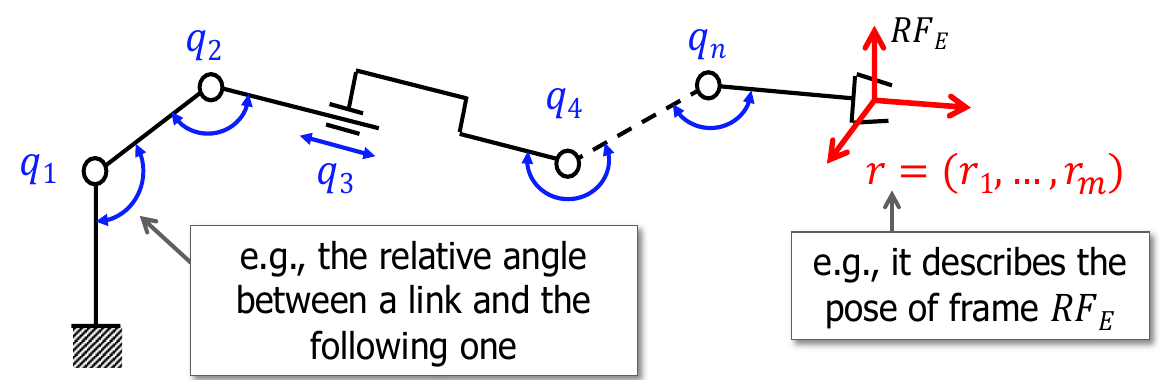
\includegraphics[width=\linewidth]{dl09_p005_chain.png}
        \end{column}
        \begin{column}{0.37\textwidth}
            \begin{itemize}
                \item number joints from the base
                \item attach local frames along the chain
                \item identify the terminal frame $RF_E$
                \item propagate motion from $q_1$ to $q_n$
            \end{itemize}
            \[
                q=[q_1,\ldots,q_n]^T
            \]
        \end{column}
    \end{columns}
\end{frame}

\begin{frame}[t]{Task Dimension Is a Modelling Choice}
    \framesubtitle{The task keeps the end-effector variables we intend to control}
    \begin{columns}[T,onlytextwidth]
        \begin{column}{0.55\textwidth}
            \begin{tabular}{ll}
                \toprule
                Task & Dimension $m$ \\
                \midrule
                planar point position & 2 \\
                spatial point position & 3 \\
                planar pose & 3 \\
                spatial pose & 6 \\
                \bottomrule
            \end{tabular}
        \end{column}
        \begin{column}{0.42\textwidth}
            \begin{block}{Typical design goal}
                \[
                    m\le n
                \]
                provides enough joint variables for an $m$-dimensional local task.
            \end{block}
            It does not guarantee global reachability, uniqueness, or freedom from singularities.
        \end{column}
    \end{columns}
\end{frame}

\begin{frame}[t]{Two Routes to Direct Kinematics}
    \framesubtitle{Inspection is efficient. Frame propagation is systematic}
    \begin{columns}[T,onlytextwidth]
        \begin{column}{0.46\textwidth}
            \begin{block}{Geometric inspection}
                \begin{itemize}
                    \item draw link vectors
                    \item project them onto axes
                    \item add relative angles
                \end{itemize}
            \end{block}
            Best for simple planar mechanisms.
        \end{column}
        \begin{column}{0.50\textwidth}
            \begin{block}{Homogeneous transforms}
                \begin{itemize}
                    \item attach a frame to every link
                    \item describe each relative motion
                    \item multiply in chain order
                \end{itemize}
            \end{block}
            \[
                {}^{0}T_n={}^{0}T_1{}^{1}T_2\cdots{}^{n-1}T_n
            \]
        \end{column}
    \end{columns}
    \medskip
    \centering
    Both routes must produce the same end-effector pose.
\end{frame}

\begin{frame}[t]{Planar 2R Direct Kinematics by Inspection}
    \framesubtitle{Project each link and add the relative rotations}
    \begin{columns}[T,onlytextwidth]
        \begin{column}{0.45\textwidth}
            \centering
            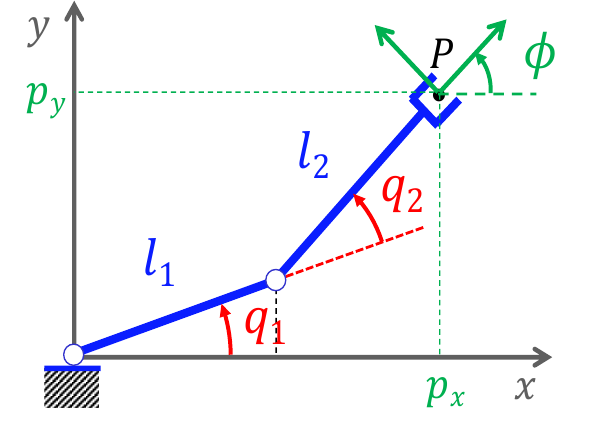
\includegraphics[width=\linewidth]{dl09_p008_2r.png}
        \end{column}
        \begin{column}{0.52\textwidth}
            \[
                \begin{aligned}
                    p_x &= l_1\cos q_1+l_2\cos(q_1+q_2),\\
                    p_y &= l_1\sin q_1+l_2\sin(q_1+q_2),\\
                    \phi &= q_1+q_2.
                \end{aligned}
            \]
            \begin{block}{Dimension check}
                The robot has $n=2$ joints but the pose vector
                $r=[p_x,p_y,\phi]^T$ has $m=3$ entries.
                They cannot all be commanded independently.
            \end{block}
        \end{column}
    \end{columns}
\end{frame}

\begin{frame}[t]{Why a Frame Convention Is Needed}
    \framesubtitle{A fixed convention makes link transforms comparable}
    \begin{columns}[T,onlytextwidth]
        \begin{column}{0.48\textwidth}
            Any consistent set of link frames can describe a robot.

            \medskip
            Arbitrary choices, however, produce parameter tables that are hard to compare and easy to misread.

            \begin{block}{Purpose of DH notation}
                Use the same four geometric parameters and the same motion order for every link.
            \end{block}
        \end{column}
        \begin{column}{0.48\textwidth}
            \[
                {}^{i-1}T_i=
                T_z(d_i)R_z(\theta_i)T_x(a_i)R_x(\alpha_i)
            \]
            \begin{block}{Video checkpoint}
                DH frame assignment. Viewing prompt: which axis must coincide with joint $i$?
            \end{block}
        \end{column}
    \end{columns}
\end{frame}

\begin{frame}[t]{DH Notation}
    \framesubtitle{Four parameters describe one relative link transform}
    \begin{columns}[T,onlytextwidth]
        \begin{column}{0.47\textwidth}
            \begin{tabular}{cl}
                \toprule
                Parameter & Motion \\
                \midrule
                $\theta_i$ & rotation about $z_{i-1}$ \\
                $d_i$ & translation along $z_{i-1}$ \\
                $a_i$ & translation along $x_i$ \\
                $\alpha_i$ & rotation about $x_i$ \\
                \bottomrule
            \end{tabular}
        \end{column}
        \begin{column}{0.50\textwidth}
            \[
                T_z(d_i)\,R_z(\theta_i)\,T_x(a_i)\,R_x(\alpha_i)
            \]
            \begin{itemize}
                \item revolute joint: $\theta_i$ varies
                \item prismatic joint: $d_i$ varies
            \end{itemize}
            \begin{block}{Convention check}
                Standard and modified DH use different orders. A table and its transform formula must use the same convention.
            \end{block}
        \end{column}
    \end{columns}
\end{frame}

\begin{frame}[t]{The 2R Arm as a Transform Chain}
    \framesubtitle{Forward kinematics assigns one pose to each joint pair}
    \centering
    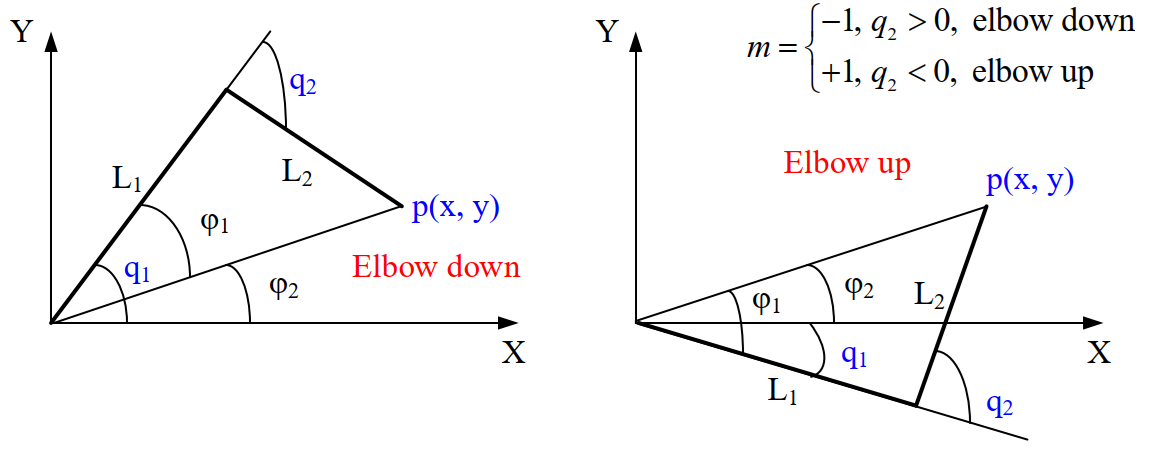
\includegraphics[width=0.88\textwidth]{kl_l1_p058_2r_branches.png}

    \smallskip
    \[
        {}^{0}T_1=R_z(q_1)T_x(l_1),
        \qquad
        {}^{1}T_2=R_z(q_2)T_x(l_2)
    \]
\end{frame}

\begin{frame}[t]{First Link Transform}
    \framesubtitle{The rotation block gives axes. The last column gives the elbow position}
    \begin{columns}[T,onlytextwidth]
        \begin{column}{0.56\textwidth}
            \[
                {}^{0}T_1=
                \begin{bmatrix}
                    c_1 & -s_1 & 0 & l_1c_1\\
                    s_1 &  c_1 & 0 & l_1s_1\\
                    0   &  0   & 1 & 0\\
                    0   &  0   & 0 & 1
                \end{bmatrix}
            \]
        \end{column}
        \begin{column}{0.40\textwidth}
            \[
                c_i=\cos q_i,
                \qquad
                s_i=\sin q_i
            \]
            \begin{block}{Read the matrix}
                The elbow coordinates are
                \[
                    (l_1c_1,l_1s_1).
                \]
            \end{block}
        \end{column}
    \end{columns}
\end{frame}

\begin{frame}[t]{Composition of Both Links}
    \framesubtitle{Matrix multiplication recovers the angle-sum terms}
    \small
    \[
        {}^{0}T_2={}^{0}T_1{}^{1}T_2=
        \begin{bmatrix}
            c_{12} & -s_{12} & 0 & l_1c_1+l_2c_{12}\\
            s_{12} &  c_{12} & 0 & l_1s_1+l_2s_{12}\\
            0      &  0      & 1 & 0\\
            0      &  0      & 0 & 1
        \end{bmatrix}
    \]
    \[
        c_{12}=\cos(q_1+q_2),
        \qquad
        s_{12}=\sin(q_1+q_2)
    \]
    \begin{block}{Composition rule}
        Relative transforms multiply in physical chain order. Reversing the factors describes a different motion.
    \end{block}
\end{frame}

\begin{frame}[t]{Geometry and Matrices Agree}
    \framesubtitle{The two derivations provide a direct implementation check}
    \begin{columns}[T,onlytextwidth]
        \begin{column}{0.48\textwidth}
            \begin{block}{From vector projection}
                \[
                    \begin{aligned}
                        p_x&=l_1c_1+l_2c_{12},\\
                        p_y&=l_1s_1+l_2s_{12},\\
                        \phi&=q_1+q_2.
                    \end{aligned}
                \]
            \end{block}
        \end{column}
        \begin{column}{0.48\textwidth}
            \begin{block}{From ${}^{0}T_2$}
                \begin{itemize}
                    \item last column gives $(p_x,p_y)$
                    \item rotation block gives $\phi$
                \end{itemize}
            \end{block}
            A mismatch usually means a frame, sign, relative-angle, or multiplication-order error.
        \end{column}
    \end{columns}
\end{frame}

\begin{frame}[t]{The Inverse Kinematics Problem}
    \framesubtitle{A desired task value defines a nonlinear equation, not a guaranteed inverse}
    \begin{block}{Given}
        A desired end-effector pose or task vector $r_d$.
    \end{block}
    \begin{block}{Find}
        Every admissible joint vector $q$ satisfying
        \[
            f_r(q)=r_d.
        \]
    \end{block}
    \begin{columns}[T,onlytextwidth]
        \begin{column}{0.31\textwidth}\centering\Large Existence\\[-1mm]\small Is $r_d$ reachable?\end{column}
        \begin{column}{0.31\textwidth}\centering\Large Multiplicity\\[-1mm]\small How many branches?\end{column}
        \begin{column}{0.31\textwidth}\centering\Large Method\\[-1mm]\small Closed form or iteration?\end{column}
    \end{columns}
\end{frame}

\begin{frame}[t]{Configuration Branches of a 6R Arm}
    \framesubtitle{Shoulder and elbow choices already create four main-arm solutions}
    \centering
    \begin{minipage}{0.23\textwidth}\centering
        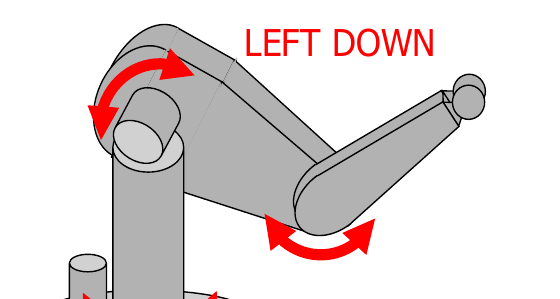
\includegraphics[width=\linewidth]{dl10_p007_left_down.png}\\[-1mm]
        \small left / elbow down
    \end{minipage}\hfill
    \begin{minipage}{0.23\textwidth}\centering
        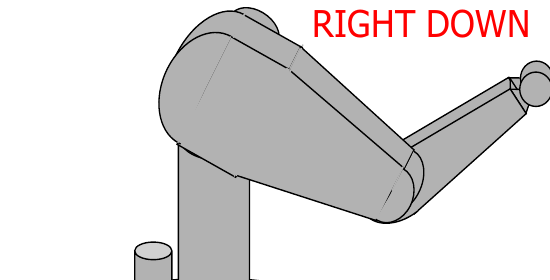
\includegraphics[width=\linewidth]{dl10_p007_right_down.png}\\[-1mm]
        \small right / elbow down
    \end{minipage}\hfill
    \begin{minipage}{0.23\textwidth}\centering
        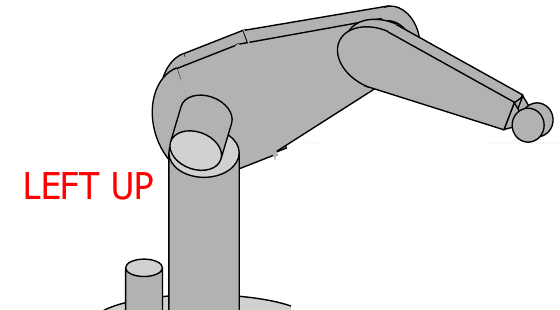
\includegraphics[width=\linewidth]{dl10_p007_left_up.png}\\[-1mm]
        \small left / elbow up
    \end{minipage}\hfill
    \begin{minipage}{0.23\textwidth}\centering
        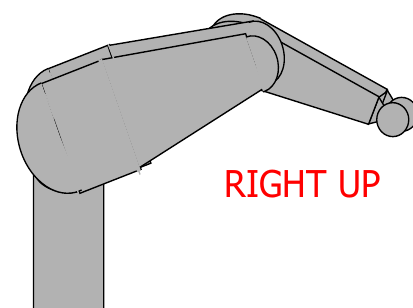
\includegraphics[width=\linewidth]{dl10_p007_right_up.png}\\[-1mm]
        \small right / elbow up
    \end{minipage}
    \bigskip
    \begin{block}{Main-arm branch count}
        \centering
        $2_{\text{shoulder}}\times2_{\text{elbow}}=4$
        regular position branches away from singularities.
    \end{block}
\end{frame}

\begin{frame}[t]{Why Four Position Branches Become Eight Poses}
    \framesubtitle{A spherical wrist adds a second orientation branch to each main-arm branch}
    \begin{columns}[T,onlytextwidth]
        \begin{column}{0.57\textwidth}
            \centering
            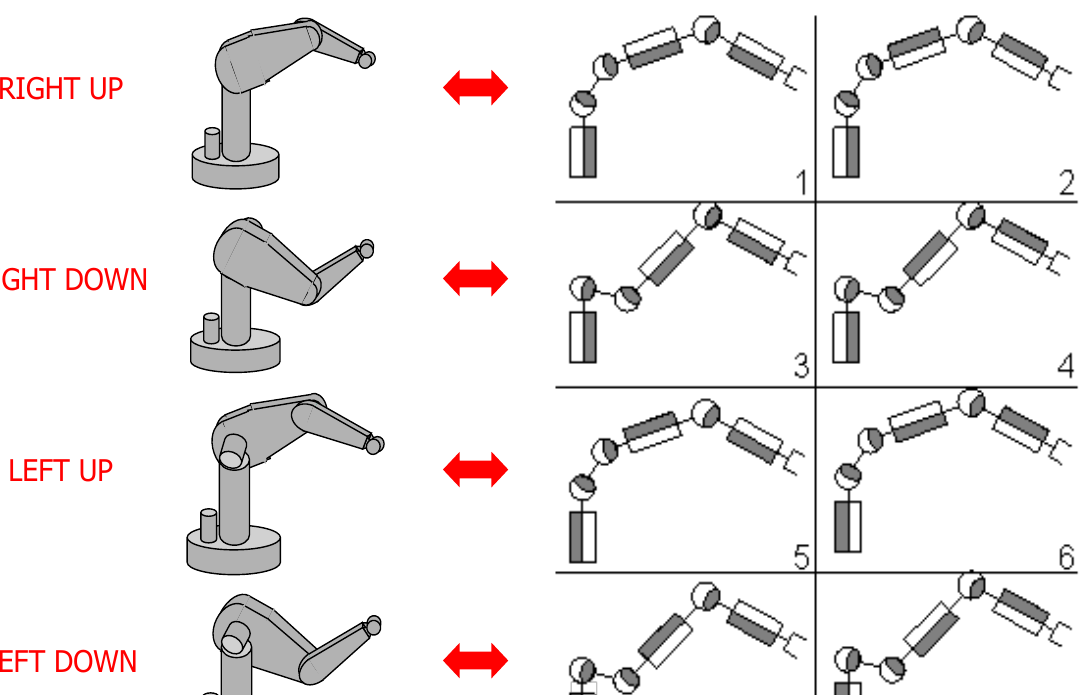
\includegraphics[width=\linewidth,height=0.62\textheight,keepaspectratio]{dl10_p008_eight_solutions.png}
        \end{column}
        \begin{column}{0.39\textwidth}
            \[
                2_{\text{shoulder}}
                \times2_{\text{elbow}}
                \times2_{\text{wrist}}=8
            \]
            \begin{itemize}
                \item same feasible nonsingular tool pose
                \item distinct joint configurations
                \item joint limits and collisions can remove branches
            \end{itemize}
        \end{column}
    \end{columns}
\end{frame}

\begin{frame}[t]{How Many IK Solutions Can Exist?}
    \framesubtitle{The count depends on robot geometry, target location, and singularity}
    \begin{columns}[T,onlytextwidth]
        \begin{column}{0.48\textwidth}
            \begin{block}{Representative regular cases}
                \begin{itemize}
                    \item planar 2R: usually two interior solutions
                    \item spatial elbow 3R: up to four position solutions
                    \item general spatial 6R: algebraic upper bound of sixteen
                \end{itemize}
            \end{block}
        \end{column}
        \begin{column}{0.48\textwidth}
            \begin{block}{Where the count changes}
                \begin{itemize}
                    \item outside the workspace: no real solution
                    \item workspace boundary: branches merge
                    \item singular set: local structure changes
                    \item constraints: mathematical branches may be infeasible
                \end{itemize}
            \end{block}
        \end{column}
    \end{columns}
    \medskip
    \centering
    \alert{Polynomial roots are not automatically real, distinct, or feasible robot poses.}
\end{frame}

\begin{frame}[t]{Turning Trigonometry into a Polynomial}
    \framesubtitle{The tangent-half-angle substitution exposes algebraic IK branches}
    \[
        a\sin\theta+b\cos\theta=c,
        \qquad
        u=\tan\frac{\theta}{2}
    \]
    \[
        \sin\theta=\frac{2u}{1+u^2},
        \qquad
        \cos\theta=\frac{1-u^2}{1+u^2}
    \]
    \begin{block}{After clearing the denominator}
        \[
            (b+c)u^2-2au-(b-c)=0.
        \]
    \end{block}
    \small
    Real roots must be mapped back to angles and checked in the original equation.
    The projective case $\theta=\pi$ corresponds to $u=\infty$ and needs separate care.
\end{frame}

\begin{frame}[t]{A 6R Robot with Sixteen Real Solutions}
    \framesubtitle{The familiar eight-branch count is not universal}
    \begin{columns}[T,onlytextwidth]
        \begin{column}{0.57\textwidth}
            \centering
            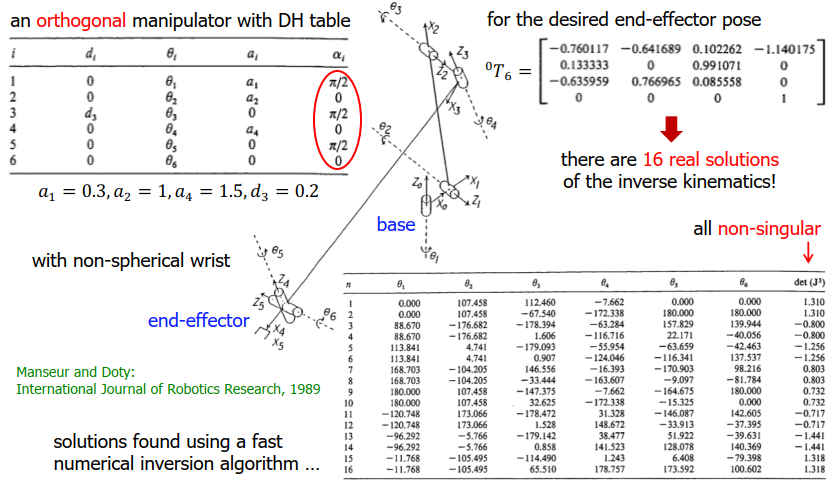
\includegraphics[width=\linewidth,height=0.66\textheight,keepaspectratio]{dl10_p013_16_solutions.png}
        \end{column}
        \begin{column}{0.39\textwidth}
            \small
            \begin{block}{Key counterexample}
                An orthogonal 6R robot without a spherical wrist can realize one desired pose with
                \textbf{16 distinct real nonsingular configurations}.
            \end{block}
            The eight-branch shoulder--elbow--wrist count is structure-specific.

            \medskip
            \scriptsize Example adapted from De Luca, \textit{Inverse Kinematics}.
        \end{column}
    \end{columns}
\end{frame}

\begin{frame}[t]{Redundancy Creates Continua of Solutions}
    \framesubtitle{A redundant task can preserve the endpoint while internal joints move}
    \begin{columns}[T,onlytextwidth]
        \begin{column}{0.58\textwidth}
            \centering
            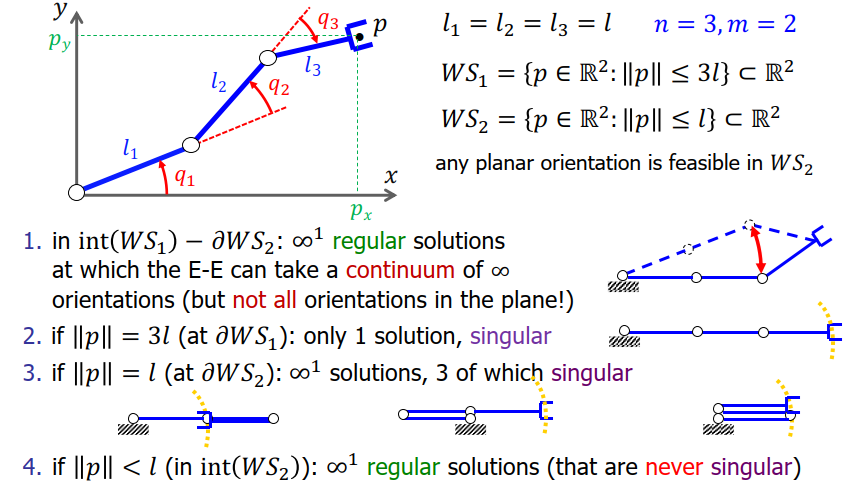
\includegraphics[width=\linewidth,height=0.64\textheight,keepaspectratio]{dl10_p014_planar_3r.png}
        \end{column}
        \begin{column}{0.38\textwidth}
            A planar 3R arm used only for point positioning has
            \[
                n=3,\qquad m=2.
            \]
            At a regular solution, the generic local solution-set dimension is
            \[
                n-m=1.
            \]
            Thus one internal degree of freedom may vary while the point stays fixed.
        \end{column}
    \end{columns}
\end{frame}

\begin{frame}[t]{Workspace of a Planar 3R Arm}
    \framesubtitle{The longest link decides whether a central hole remains}
    \begin{columns}[T,onlytextwidth]
        \begin{column}{0.57\textwidth}
            \centering
            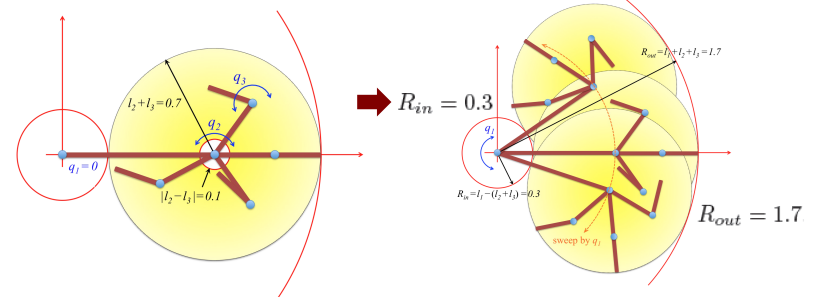
\includegraphics[width=\linewidth,height=0.61\textheight,keepaspectratio]{dl10_p015_workspace_cases.png}
        \end{column}
        \begin{column}{0.39\textwidth}
            \small
            Sort the lengths as $l_{\min}\le l_{\mathrm{med}}\le l_{\max}$.
            \[
                R_{\mathrm{out}}=l_1+l_2+l_3
            \]
            \[
                R_{\mathrm{in}}=
                \max\!\left\{0,\,
                l_{\max}-l_{\mathrm{med}}-l_{\min}\right\}
            \]
            $R_{\mathrm{in}}>0$ creates a central unreachable disk; otherwise the workspace includes the base.
        \end{column}
    \end{columns}
\end{frame}

\begin{frame}[t]{Multiplicity by Dimension Count}
    \framesubtitle{Task dimension and Jacobian rank predict the local solution structure}
    \small
    \begin{columns}[T,onlytextwidth]
        \begin{column}{0.46\textwidth}
            \begin{block}{Square task: $m=n$}
                Regular IK solutions are locally isolated and are usually finite in number.
            \end{block}
        \end{column}
        \begin{column}{0.50\textwidth}
            \begin{block}{Redundant task: $m<n$}
                Regular solutions generically form a local set of dimension
                \[
                    n-m.
                \]
            \end{block}
        \end{column}
    \end{columns}
    \medskip
    \begin{block}{A singularity changes the local structure}
        \[
            \operatorname{rank}J_r(q)<m,
            \qquad
            J_r(q)=\frac{\partial f_r(q)}{\partial q}.
        \]
    \end{block}
\end{frame}

\begin{frame}[t]{Self-Motion of an 8R Arm}
    \framesubtitle{Redundancy changes internal posture while preserving the tool pose}
    \begin{columns}[T,onlytextwidth]
        \begin{column}{0.60\textwidth}
            \centering
            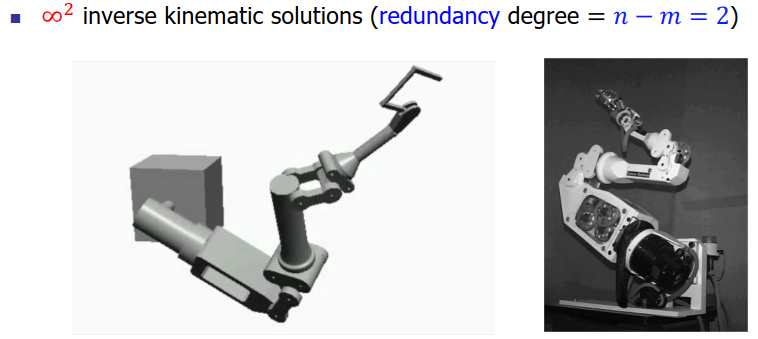
\includegraphics[width=\linewidth,height=0.57\textheight,keepaspectratio]{dl10_p017_dexter.png}
        \end{column}
        \begin{column}{0.36\textwidth}
            For a full spatial pose,
            \[
                n=8,\quad m=6,
                \qquad n-m=2.
            \]
            A two-dimensional family of joint motions can preserve the same tool pose at regular configurations.
        \end{column}
    \end{columns}
    \medskip
    \begin{block}{Video checkpoint}
        Observe how Dexter changes its internal posture while preserving the tool pose.
    \end{block}
\end{frame}

\begin{frame}[t]{Analytical or Numerical IK?}
    \framesubtitle{Choose the method by robot structure, constraints, and required output}
    \begin{columns}[T,onlytextwidth]
        \begin{column}{0.48\textwidth}
            \begin{block}{Analytical methods}
                \begin{itemize}
                    \item fast evaluation after derivation
                    \item expose discrete solution branches
                    \item depend on exploitable geometry
                \end{itemize}
            \end{block}
            Pieper-type conditions are sufficient geometric conditions for closed-form IK of many 6R arms.
        \end{column}
        \begin{column}{0.48\textwidth}
            \begin{block}{Numerical methods}
                \begin{itemize}
                    \item general across robot geometries
                    \item natural for redundant tasks
                    \item return a solution near the initial guess
                \end{itemize}
            \end{block}
            Constraints, singularities, and convergence must be handled explicitly in either approach.
        \end{column}
    \end{columns}
\end{frame}

\begin{frame}[t]{Planar 2R IK: Solve for the Elbow}
    \framesubtitle{One cosine equation gives reachability and both elbow branches}
    \begin{columns}[T,onlytextwidth]
        \begin{column}{0.43\textwidth}
            \centering
            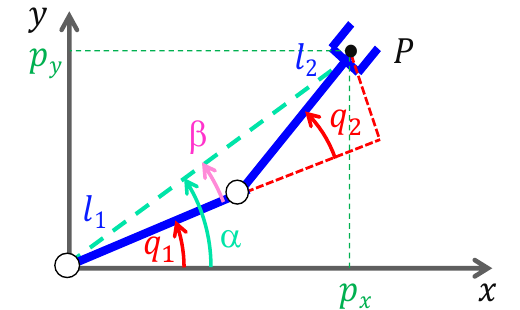
\includegraphics[width=\linewidth,height=0.60\textheight,keepaspectratio]{dl10_p020_alpha_beta_geometry.png}
        \end{column}
        \begin{column}{0.53\textwidth}
            Square and add the two forward-kinematics equations:
            \[
                c_2=\frac{p_x^2+p_y^2-l_1^2-l_2^2}{2l_1l_2}.
            \]
            \[
                s_2=\pm\sqrt{1-c_2^2},
                \qquad
                q_2=\operatorname{atan2}(s_2,c_2).
            \]
            \begin{block}{Reachability test}
                $|c_2|>1$ means the desired point lies outside the workspace.
            \end{block}
        \end{column}
    \end{columns}
\end{frame}

\begin{frame}[t]{Planar 2R IK: Solve for the Shoulder}
    \framesubtitle{Target bearing minus triangle angle completes each elbow branch}
    \begin{columns}[T,onlytextwidth]
        \begin{column}{0.47\textwidth}
            Define the target bearing
            \[
                \alpha=\operatorname{atan2}(p_y,p_x).
            \]
            Then, for each chosen sign of $s_2$,
            \[
                \begin{aligned}
                q_1={}&\operatorname{atan2}(p_y,p_x)\\
                       &-\operatorname{atan2}(l_2s_2,l_1+l_2c_2).
                \end{aligned}
            \]
            Normalize the angle difference to the course convention.
        \end{column}
        \begin{column}{0.49\textwidth}
            \centering
            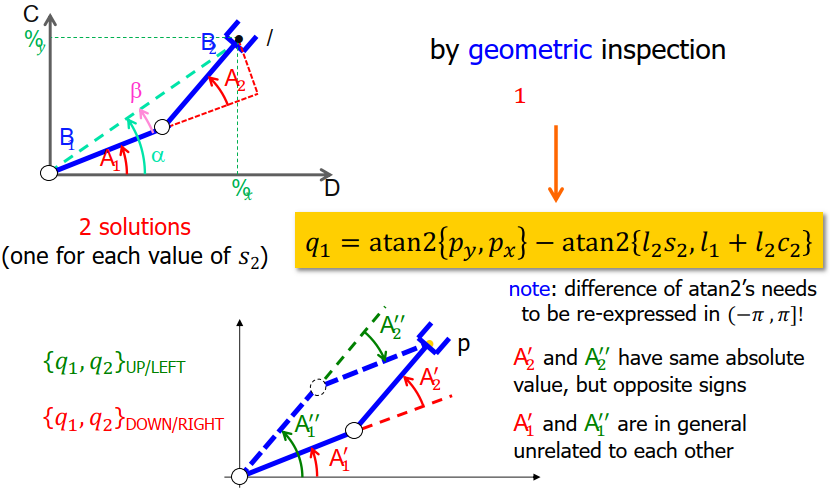
\includegraphics[width=\linewidth,height=0.62\textheight,keepaspectratio]{dl10_p020_alpha_beta_geom4.png}
        \end{column}
    \end{columns}
\end{frame}

\begin{frame}[t]{Planar 2R IK: Algebraic Shoulder Solution}
    \framesubtitle{A linear system reproduces the geometric formula and reveals a singular exception}
    \footnotesize
    \[
        \begin{bmatrix}p_x\\p_y\end{bmatrix}=
        \begin{bmatrix}
            l_1+l_2c_2 & -l_2s_2\\
            l_2s_2 & l_1+l_2c_2
        \end{bmatrix}
        \begin{bmatrix}c_1\\s_1\end{bmatrix}.
    \]
    \[
        D=(l_1+l_2c_2)^2+(l_2s_2)^2
        =l_1^2+l_2^2+2l_1l_2c_2.
    \]
    For $D>0$, solve for $c_1,s_1$ and recover
    \[
        q_1=\operatorname{atan2}(s_1,c_1).
    \]
    \begin{block}{Guard before division}
        If $l_1=l_2$, $c_2=-1$, and the target is the origin, then $D=0$ and $q_1$ is undetermined.
    \end{block}
\end{frame}

\begin{frame}[t]{Inverse Kinematics of a Polar RRP Arm}
    \framesubtitle{Radial extension, elevation, and azimuth can be solved in sequence}
    \begin{columns}[T,onlytextwidth]
        \begin{column}{0.46\textwidth}
            \centering
            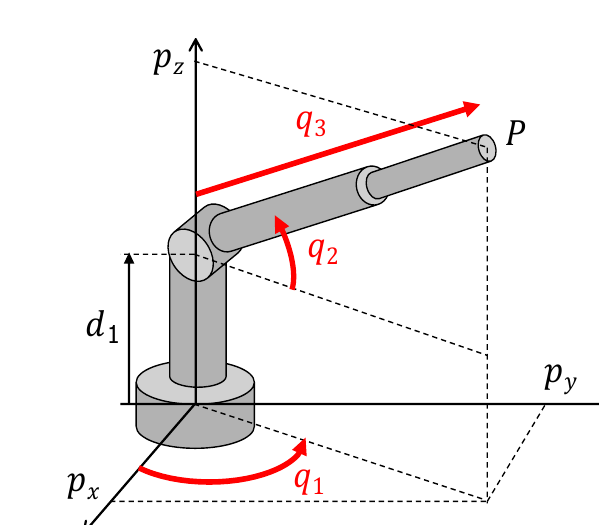
\includegraphics[width=\linewidth,height=0.64\textheight,keepaspectratio]{dl10_p022_rrp.png}
        \end{column}
        \begin{column}{0.50\textwidth}
            \small
            \[
                q_3=\sqrt{p_x^2+p_y^2+(p_z-d_1)^2}
            \]
            \[
                q_2=\operatorname{atan2}\!\left(
                p_z-d_1,\sqrt{p_x^2+p_y^2}\right)
            \]
            \[
                q_1=\operatorname{atan2}(p_y,p_x)
            \]
            \begin{block}{Undefined-angle cases}
                Check $q_3=0$ and the axis case $p_x=p_y=0$ before evaluating angles.
            \end{block}
        \end{column}
    \end{columns}
\end{frame}

\begin{frame}[t]{Geometry of a Spatial 3R Elbow Arm}
    \framesubtitle{Facing/backing and elbow up/down produce four regular position branches}
    \begin{columns}[T,onlytextwidth]
        \begin{column}{0.59\textwidth}
            \centering
            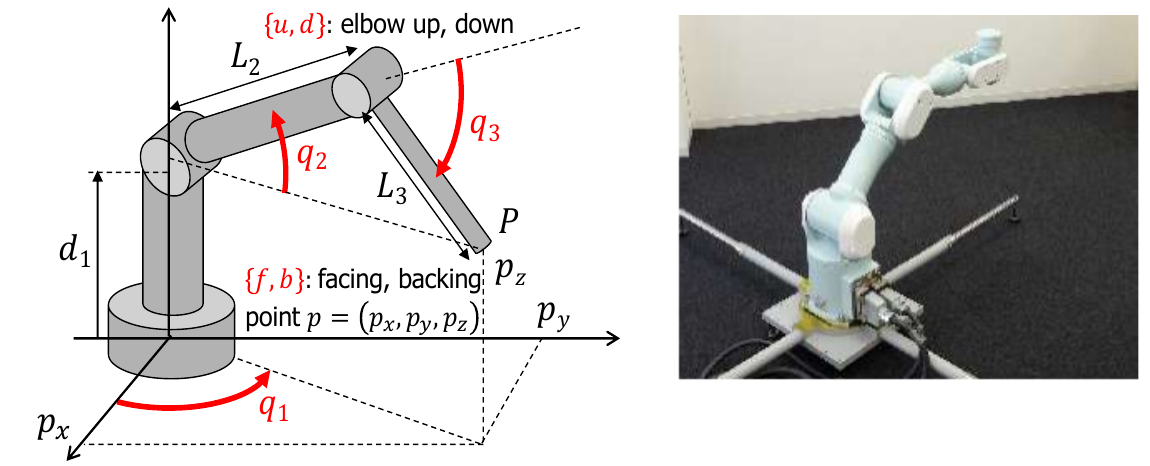
\includegraphics[width=\linewidth,height=0.64\textheight,keepaspectratio]{dl10_p023_elbow_arm.png}
        \end{column}
        \begin{column}{0.37\textwidth}
            For a symmetric arm without offsets:
            \begin{itemize}
                \item $q_1$: facing or backing branch
                \item $q_3$: elbow up or down branch
                \item $q_2$: completes each pair
            \end{itemize}
            \[
                2_{\text{base}}\times2_{\text{elbow}}=4
            \]
            regular solutions in the interior of the workspace, away from the base axis.
        \end{column}
    \end{columns}
\end{frame}

\begin{frame}[t]{Spatial 3R IK: Solve the Elbow Angle}
    \framesubtitle{Distance from the shoulder gives the same cosine-law structure as planar 2R}
    \[
        R^2=p_x^2+p_y^2+(p_z-d_1)^2,
        \qquad
        c_3=\frac{R^2-L_2^2-L_3^2}{2L_2L_3}.
    \]
    \begin{block}{Two elbow branches}
        \[
            s_3=\pm\sqrt{1-c_3^2},
            \qquad
            q_3=\operatorname{atan2}(s_3,c_3).
        \]
        The positive and negative signs give the elbow-up and elbow-down configurations.
    \end{block}
    \begin{block}{First gate}
        If $|c_3|>1$, the desired point is outside the spherical-shell workspace.
    \end{block}
\end{frame}

\begin{frame}[t]{Spatial 3R IK: Solve the Base Angle}
    \framesubtitle{The two base branches view the same radial line from opposite directions}
    When $p_x^2+p_y^2>0$, define
    \[
        q_1^{(f)}=\operatorname{atan2}(p_y,p_x),
        \qquad
        q_1^{(b)}=\operatorname{atan2}(-p_y,-p_x).
    \]
    \begin{columns}[T,onlytextwidth]
        \begin{column}{0.47\textwidth}
            \begin{block}{Facing branch}
                The signed radial coordinate
                \[
                    \rho=c_1p_x+s_1p_y
                \]
                is positive.
            \end{block}
        \end{column}
        \begin{column}{0.47\textwidth}
            \begin{block}{Backing branch}
                The same expression for $\rho$ is negative, changing the shoulder solution.
            \end{block}
        \end{column}
    \end{columns}
    \medskip
    On the base axis, $p_x=p_y=0$ and $q_1$ is undetermined: infinitely many base angles represent the same point.
\end{frame}

\begin{frame}[t]{Spatial 3R IK: Complete the Shoulder Angle}
    \framesubtitle{A $2\times2$ system determines $q_2$ for each base--elbow branch pair}
    Let
    \[
        \rho=c_1p_x+s_1p_y,
        \qquad h=p_z-d_1.
    \]
    Then
    \[
        \begin{bmatrix}
            L_2+L_3c_3 & -L_3s_3\\
            L_3s_3 & L_2+L_3c_3
        \end{bmatrix}
        \begin{bmatrix}c_2\\s_2\end{bmatrix}
        =
        \begin{bmatrix}\rho\\h\end{bmatrix}.
    \]
    Solve the system and recover
    \[
        q_2=\operatorname{atan2}(s_2,c_2).
    \]
    Each choice of $q_1$ and $q_3$ must be propagated into this equation before $q_2$ is evaluated.
\end{frame}

\begin{frame}[t]{Branch Bookkeeping for the 3R Elbow Arm}
    \framesubtitle{A solution is a consistent tuple, not an independent choice for each joint}
    \centering
    \small
    \begin{tabular}{c|cc}
        \toprule
        & elbow up $q_3^{(u)}$ & elbow down $q_3^{(d)}$ \\
        \midrule
        facing $q_1^{(f)}$ & solve matching $q_2$ & solve matching $q_2$ \\
        backing $q_1^{(b)}$ & solve matching $q_2$ & solve matching $q_2$ \\
        \bottomrule
    \end{tabular}
    \medskip
    \begin{block}{For each leaf}
        Substitute its $q_1$ and $q_3$ into the shoulder system, solve one matching $q_2$, then verify the complete tuple by forward kinematics.
    \end{block}
    Branches merge or become undefined on workspace boundaries and singular axes.
\end{frame}

\begin{frame}[t]{Spherical-Wrist Decoupling}
    \framesubtitle{Intersecting wrist axes separate position IK from orientation IK}
    \begin{columns}[T,onlytextwidth]
        \begin{column}{0.57\textwidth}
            \centering
            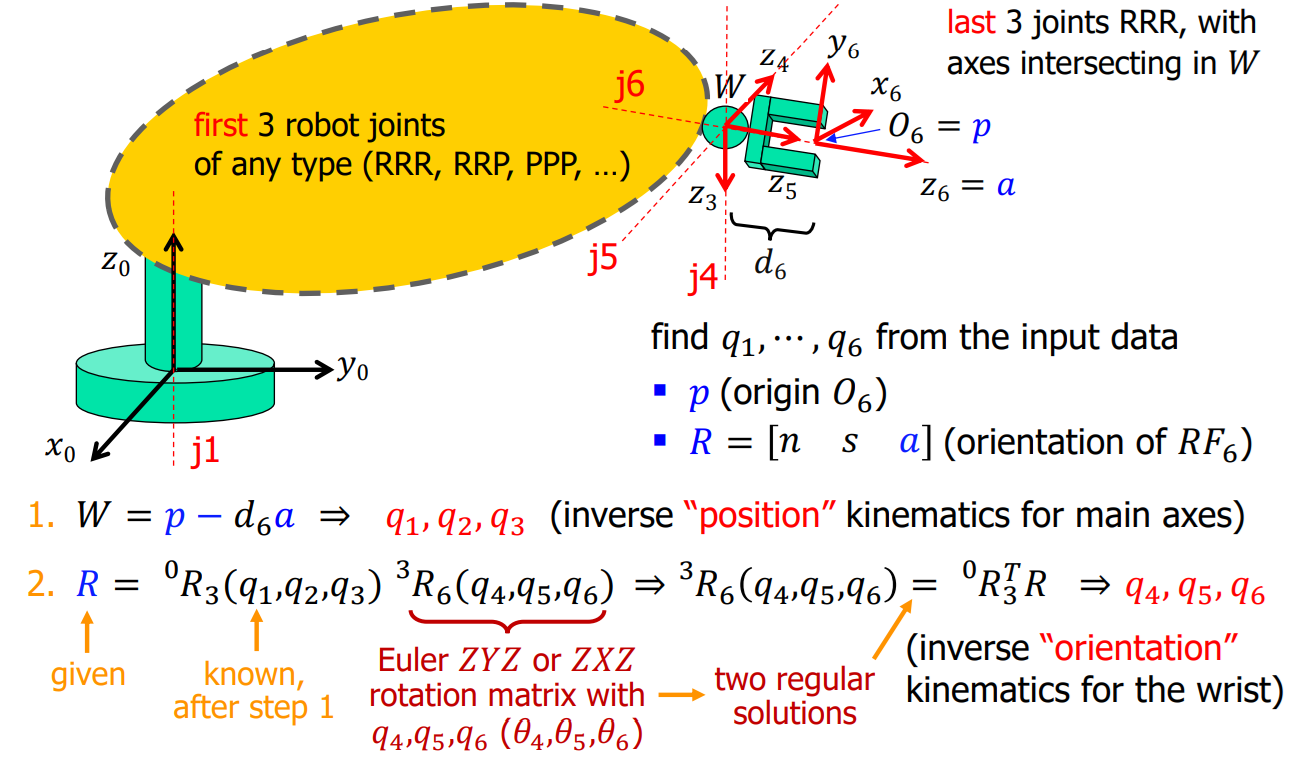
\includegraphics[width=\linewidth,height=0.63\textheight,keepaspectratio]{dl10_p027_spherical_wrist.png}
        \end{column}
        \begin{column}{0.39\textwidth}
            The last three rotation axes intersect at the wrist center $W$.
            \[
                W=p-d_6a
            \]
            where $p$ is the tool origin and $a$ is the tool $z$ axis.
            \begin{enumerate}
                \item solve $q_1,q_2,q_3$ from $W$
                \item solve $q_4,q_5,q_6$ from orientation
            \end{enumerate}
        \end{column}
    \end{columns}
\end{frame}

\begin{frame}[t]{Position First, Orientation Second}
    \framesubtitle{The first-stage branch selects the rotation matrix used by the wrist stage}
    \begin{columns}[T,onlytextwidth]
        \begin{column}{0.46\textwidth}
            \begin{block}{1. Main-arm position IK}
                \[
                    W=p-d_6a
                \]
                Find every feasible tuple $(q_1,q_2,q_3)$ placing the wrist center at $W$.
            \end{block}
        \end{column}
        \begin{column}{0.50\textwidth}
            \begin{block}{2. Wrist orientation IK}
                For each main-arm tuple, compute
                \[
                    {}^{3}R_6=({}^{0}R_3)^T{}^{0}R_6.
                \]
                Extract $(q_4,q_5,q_6)$ as Euler angles, including both regular wrist branches.
            \end{block}
        \end{column}
    \end{columns}
    \bigskip
    \centering
    \alert{Orientation solutions cannot be mixed across different main-arm branches.}
\end{frame}

\begin{frame}[t]{Closed-Form IK of the PUMA 600}
    \framesubtitle{A spherical wrist makes the eight regular branches explicit}
    \begin{columns}[T,onlytextwidth]
        \begin{column}{0.60\textwidth}
            \centering
            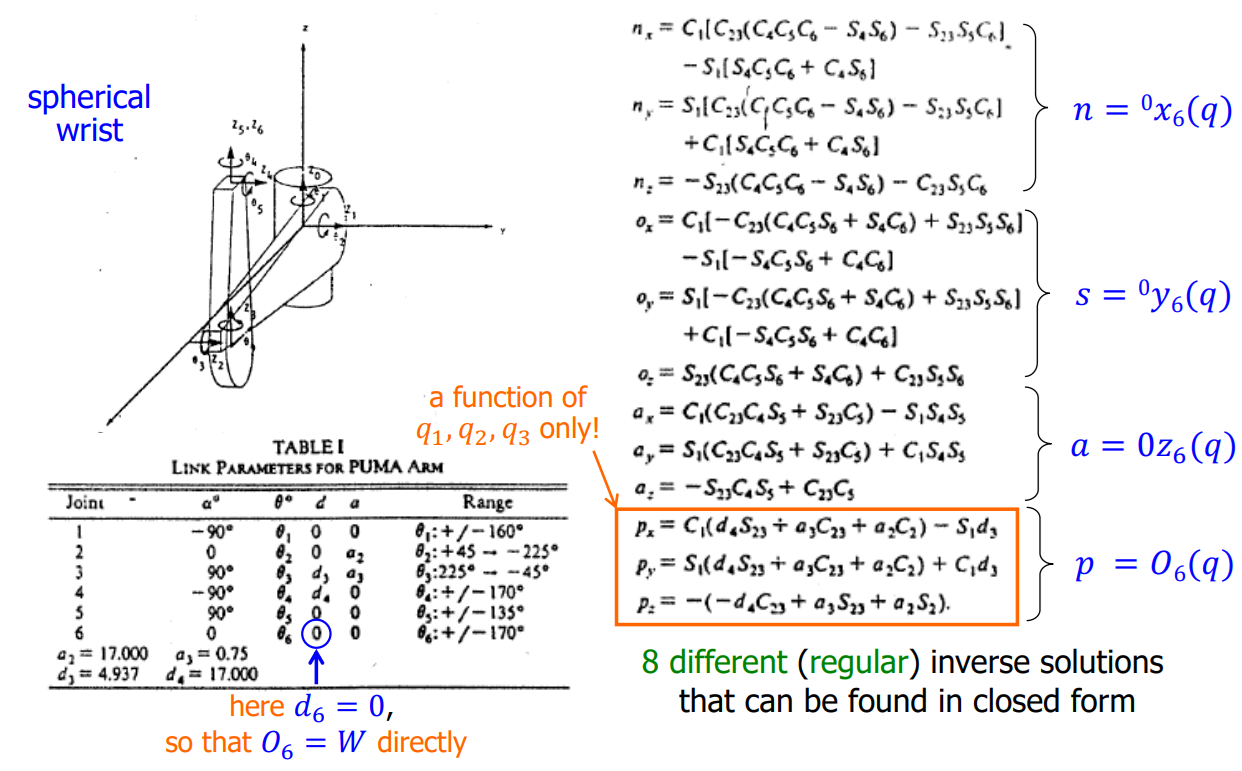
\includegraphics[width=\linewidth,height=0.65\textheight,keepaspectratio]{dl10_p028_puma.png}
        \end{column}
        \begin{column}{0.36\textwidth}
            For this geometry, $d_6=0$ and the tool origin coincides with the wrist center.
            \[
                2_{\text{shoulder}}
                \times2_{\text{elbow}}
                \times2_{\text{wrist}}=8
            \]
            regular closed-form inverse solutions.

            \medskip
            Joint limits, collisions, and singular poses still require filtering.
        \end{column}
    \end{columns}
\end{frame}

\begin{frame}[t]{Forward Chain of a 6-DOF Industrial Robot}
    \framesubtitle{Separate the main arm, spherical wrist, and external frame transforms}
    \begin{columns}[T,onlytextwidth]
        \begin{column}{0.56\textwidth}
            \centering
            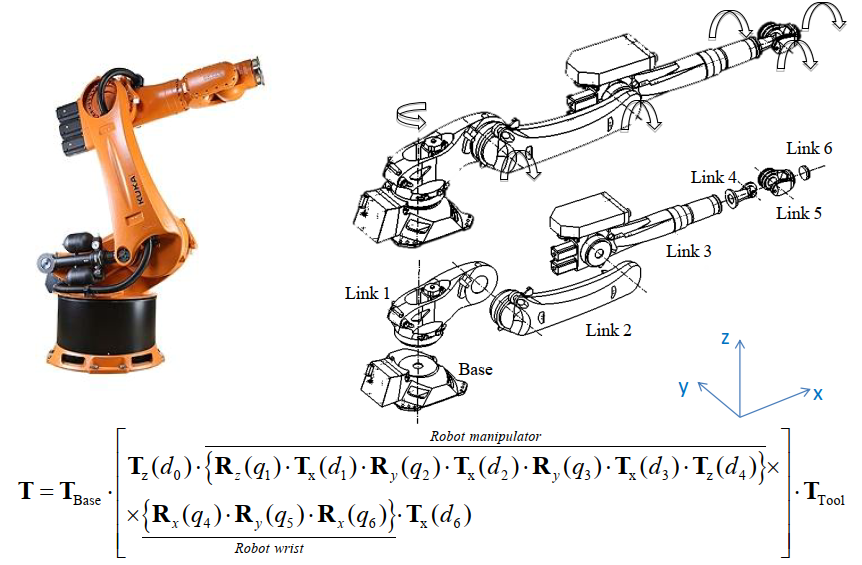
\includegraphics[width=\linewidth,height=0.62\textheight,keepaspectratio]{kl_l1_p062_robot_chain.png}
        \end{column}
        \begin{column}{0.40\textwidth}
            \small
            \[
                \begin{aligned}
                T={}&T_{\mathrm{Base}}\,T_{123}(q_1,q_2,q_3)\\
                   &\cdot T_{456}(q_4,q_5,q_6)\,T_{\mathrm{Tool}}.
                \end{aligned}
            \]
            \begin{block}{Structural split}
                \begin{itemize}
                    \item joints 1--3 place the wrist center
                    \item joints 4--6 orient the tool
                    \item base and tool transforms convert external conventions
                \end{itemize}
            \end{block}
        \end{column}
    \end{columns}
\end{frame}

\begin{frame}[t]{Pieper's Step-by-Step Procedure}
    \framesubtitle{Use wrist-center geometry first, then solve the remaining rotation}
    \begin{columns}[T,onlytextwidth]
        \begin{column}{0.65\textwidth}
            \small
            \begin{enumerate}
                \item express the desired tool pose as ${}^{0}T_6$
                \item compute the wrist center $P_c=p-d_6a$
                \item set $P_c$ equal to the position from ${}^{0}T_3(q_1,q_2,q_3)$
                \item solve every main-arm branch $(q_1,q_2,q_3)$
                \item compute ${}^{3}R_6=({}^{0}R_3)^T{}^{0}R_6$
                \item solve every wrist branch $(q_4,q_5,q_6)$
                \item preserve branch correspondence and filter constraints
            \end{enumerate}
        \end{column}
        \begin{column}{0.31\textwidth}
            \centering
            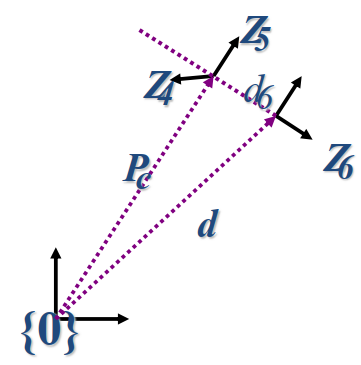
\includegraphics[width=\linewidth,height=0.61\textheight,keepaspectratio]{kl_l1_p063_wrist_center_geom.png}
        \end{column}
    \end{columns}
\end{frame}

\begin{frame}[t]{Normalize Base, Tool, and Link Offsets}
    \framesubtitle{Convert the requested pose into the transform used by the internal kinematic model}
    \begin{columns}[T,onlytextwidth]
        \begin{column}{0.49\textwidth}
            \centering
            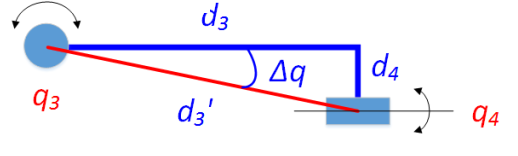
\includegraphics[width=\linewidth]{kl_l1_p064_offset_geom4.png}
            \[
                d_3'=\sqrt{d_3^2+d_4^2},
                \qquad
                \Delta q=\operatorname{atan2}(d_4,d_3).
            \]
        \end{column}
        \begin{column}{0.47\textwidth}
            Remove known external transforms before solving joint variables:
            \[
                T_0=T_z^{-1}(d_0),
                T_{\mathrm{Base}}^{-1},
                T,T_{\mathrm{Tool}}^{-1},
                T_x^{-1}(d_6).
            \]
            Absorb the perpendicular offset into the effective link length $d_3'$ and angle shift $\Delta q$.
        \end{column}
    \end{columns}
    \medskip
    \centering
    \alert{One normalized target keeps frame conventions out of the branch algebra.}
\end{frame}

\begin{frame}[t]{Solve the Main Arm}
    \framesubtitle{After normalization, the position equations reduce to a planar 2-link problem}
    Let the normalized target position be $(x',y',z')$ and define
    \[
        \rho=\pm\sqrt{x'^2+y'^2}.
    \]
    \begin{columns}[T,onlytextwidth]
        \begin{column}{0.47\textwidth}
            \begin{block}{Base branch}
                \[
                    q_1=\operatorname{atan2}(y',x')
                \]
                for one radial sign; add the backing branch for the opposite sign.
            \end{block}
        \end{column}
        \begin{column}{0.49\textwidth}
            \begin{block}{Shoulder--elbow plane}
                \[
                    \begin{aligned}
                    \rho&=d_2\cos q_2+d_3'\cos(q_2+q_3+\Delta q),\\
                    -z'&=d_2\sin q_2+d_3'\sin(q_2+q_3+\Delta q).
                    \end{aligned}
                \]
                Solve exactly as planar 2R IK.
            \end{block}
        \end{column}
    \end{columns}
    If $x'=y'=0$, the base angle is undetermined and must be handled as a singular case.
\end{frame}

\begin{frame}[t]{Solve the Robot Wrist}
    \framesubtitle{Each main-arm branch defines a residual rotation for the last three joints}
    \[
        T_{456}=T_{123}^{-1}T_0,
        \qquad
        R_{456}=R_x(q_4)R_y(q_5)R_x(q_6).
    \]
    \begin{columns}[T,onlytextwidth]
        \begin{column}{0.47\textwidth}
            \begin{block}{Regular wrist}
                Extract $q_5$ from a diagonal entry, then use paired off-diagonal entries in $\operatorname{atan2}$ to obtain $q_4$ and $q_6$.

                \medskip
                Two regular Euler-angle branches represent the same residual rotation.
            \end{block}
        \end{column}
        \begin{column}{0.49\textwidth}
            \begin{block}{Wrist singularity}
                When $\sin q_5=0$, the first and third wrist axes align. Only a sum or difference of $q_4$ and $q_6$ is observable.

                \medskip
                Choose one free angle explicitly and compute the other.
            \end{block}
        \end{column}
    \end{columns}
\end{frame}

\begin{frame}[t]{Numerical IK with Newton's Method}
    \framesubtitle{Linearize the task map at the current joint estimate}
    Let
    \[
        e_k=r_d-f_r(q_k),
        \qquad
        J_k=J_r(q_k).
    \]
    For a square nonsingular task, the Newton update is
    \[
        q_{k+1}=q_k+J_k^{-1}e_k.
    \]
    \begin{columns}[T,onlytextwidth]
        \begin{column}{0.47\textwidth}
            \begin{block}{Why it can be fast}
                Near a regular solution, the local linear model is accurate and convergence can be quadratic.
            \end{block}
        \end{column}
        \begin{column}{0.49\textwidth}
            \begin{block}{Redundant task}
                For $m<n$, replace the inverse with a pseudoinverse:
                \[
                    \Delta q=J_k^{\dagger}e_k.
                \]
            \end{block}
        \end{column}
    \end{columns}
\end{frame}

\begin{frame}[t]{When Newton's Method Succeeds or Fails}
    \framesubtitle{The initial guess, conditioning, and step policy determine the observed branch}
    \begin{columns}[T,onlytextwidth]
        \begin{column}{0.48\textwidth}
            \begin{block}{Reliable regime}
                \begin{itemize}
                    \item $q_0$ lies near a regular solution
                    \item $J_r(q)$ is well conditioned
                    \item the local linear step reduces task error
                \end{itemize}
            \end{block}
        \end{column}
        \begin{column}{0.48\textwidth}
            \begin{block}{Common failure modes}
                \begin{itemize}
                    \item distant initial guess
                    \item singular or nearly singular Jacobian
                    \item step leaves joint limits or overshoots
                    \item iteration converges to an unwanted branch
                \end{itemize}
            \end{block}
        \end{column}
    \end{columns}
    \bigskip
    \centering
    A numerical solver normally finds \emph{one nearby solution}; multiple seeds are needed to explore multiple branches.
\end{frame}

\begin{frame}[t]{Gradient-Descent IK}
    \framesubtitle{Jacobian transpose gives a descent direction without matrix inversion}
    Define the squared task error
    \[
        H(q)=\frac{1}{2}\left\|r_d-f_r(q)\right\|^2.
    \]
    Since
    \[
        \nabla_q H(q)=-J_r^T(q)\left[r_d-f_r(q)\right],
    \]
    steepest descent gives
    \[
        q_{k+1}=q_k+\alpha J_r^T(q_k)
        \left[r_d-f_r(q_k)\right],
        \qquad \alpha>0.
    \]
    \begin{block}{Step-size trade-off}
        Too large an $\alpha$ may increase the error or miss the minimum; too small an $\alpha$ makes convergence very slow.
    \end{block}
\end{frame}

\begin{frame}[t]{Workspace of an Industrial Manipulator}
    \framesubtitle{A planar cross-section swept by the base joint creates a three-dimensional volume}
    \begin{columns}[T,onlytextwidth]
        \begin{column}{0.59\textwidth}
            \centering
            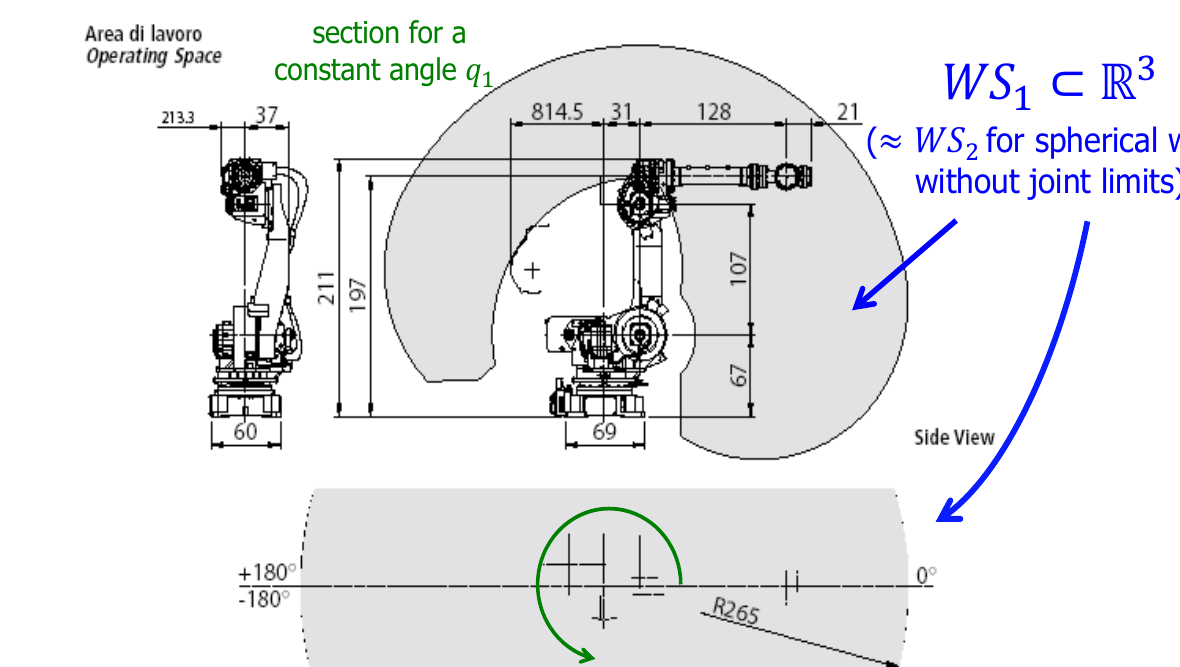
\includegraphics[width=\linewidth,height=0.65\textheight,keepaspectratio]{dl10_p005_fanuc_workspace.png}
        \end{column}
        \begin{column}{0.37\textwidth}
            \small
            Fix the base angle $q_1$ to inspect one meridional workspace section.

            \medskip
            Rotating that section about the base axis sweeps the position workspace
            \[
                WS_p\subset\mathbb{R}^3.
            \]
            With a spherical wrist and no joint limits, this approximates the wrist-center workspace.
        \end{column}
    \end{columns}
\end{frame}

\begin{frame}[t]{Planar 2R Workspace and Branch Count}
    \framesubtitle{Reachability and IK multiplicity are two views of the same geometry}
    \begin{columns}[T,onlytextwidth]
        \begin{column}{0.58\textwidth}
            \centering
            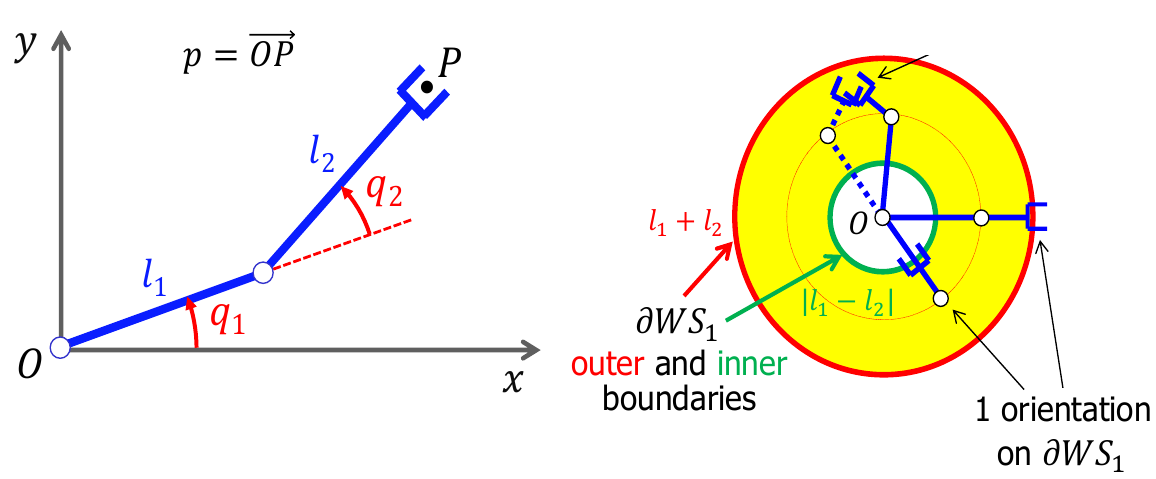
\includegraphics[width=\linewidth,height=0.63\textheight,keepaspectratio]{dl10_p006_2r_workspace.png}
        \end{column}
        \begin{column}{0.38\textwidth}
            With $\rho=\sqrt{p_x^2+p_y^2}$,
            \[
                |l_1-l_2|\le\rho\le l_1+l_2.
            \]
            \begin{itemize}
                \item interior: two elbow branches
                \item inner or outer boundary: one merged branch
                \item outside: no real solution
            \end{itemize}
            If $l_1=l_2$ and $\rho=0$, infinitely many joint pairs fold to the origin.
        \end{column}
    \end{columns}
\end{frame}

\begin{frame}[t]{Reference Materials}
    \begin{itemize}
        \item A. De Luca --- 09 DirectKinematics
        \item A. Klimchik --- L1 Introduction
        \item A. De Luca --- 10 InverseKinematics
    \end{itemize}
\end{frame}


\fbckg{fibeamer/figs/last_page.png}
\frame[plain]{}

\end{document}
